%% ----------------------------------------------------------------
%% Introduction.tex
%% ---------------------------------------------------------------- 
\chapter{Introduction} \label{Chapter:Introduction}

%This dissertation was a part of my master’s project at the Univerisity of Southampton, under the guidance of Dr. Sasan Barak. The project focuses on financial data science within cryptocurrency markets. 

Financial markets, like cryptocurrencies, are widely considered to be non-stationary~\cite{Schmitt_2013,Lo} as their statistical properties—including volatility, correlations, and return distributions change frequently over time.
The non-stationarity brings a major challenge for trading and risk management, as optimised strategies under one regime often fail when market condition changes~\cite{10.1093/rfs/15.4.1137}. 

Traditional trading strategies generally assume a stable market environment, therefore the strategy performance probably varies across different market states. For example, a momentum-based method may perform well in a trending market but much worse in volatile periods~\cite{MOSKOWITZ2012228}; Similarly, risk measures calculated under a volatility regime may underestimate the risk during a crisis regime~\cite{HAMILTON1994307}.

To address the challenges from market non-stationarity, a range of methods are developed, such as Markov switching models~\cite{hamilton1989new}, and clustering approaches~\cite{10.1093/rfs/15.4.1137}. More recently, mathematical tools from rough path theory have given rise to signature methods~\cite{ chevyrev2025primersignaturemethodmachine,issa2023nonparametriconlinemarketregime}, which are capable of extracting rich path-wise features from time series data. Combined with clustering, these features can be used to identify distinct market regimes, such as bull, bear, and neutral phases.

In this study, we applied signature methods~\cite{Lyons1998, chevyrev2025primersignaturemethodmachine,issa2023nonparametriconlinemarketregime} to extract path-wise features from BTC prices and perform walk-forward clustering to obtain regimes.

Lead–lag refers to directed, time-shifted dependence in returns across assets. A number of literature develops practical estimators and documents this structure via futures–spot studies, high-frequency (Hayashi–Yoshida–style) measures, and daily directed-network clustering, which shows economic value for cross-sectional trading~\cite{BROOKS200131,huth2012leadlag,bennett2022leadlag}. Building on this, we implement a cross-sectional lead–lag hedge~\cite{lyons2002system, gatheral2018volatility} as our baseline, and then overlay our previously estimated regime signal to adjust position signs and scale exposures.

Given our motivation for this study, this study attempted to address the following research question:

\noindent\textbf{RQ1:} How can market regimes be detected in a using signature–kernel \emph{path-wise} features of an asset?\\
\noindent\textbf{RQ2:} Holding market participation fixed, do regime-conditioned signature lead–lag hedges improve risk-adjusted performance over an unconditional baseline? 

\noindent\textbf{RQ3:} How sensitive are the results to key hyperparameters and trading frictions—like path segmentation, voting windows, and transaction costs?

In relation with the questions, the following objectives are aimed to achieve in this study:

\noindent\textbf{RO1:} Develop a data-driven regime detector based on signature-kernel MMD with strict walk-forward clustering and medoid semantics, producing daily bull/neutral/bear labels without look-ahead.\\
\noindent\textbf{RO2:} Build (i) a baseline signature-based lead–lag portfolio (long followers / short leaders) and (ii) a regime-aware overlay that preserves the hedge while routing names by their signed relation to a BTC anchor.\\
\textbf{RO3:} Evaluate performance with headline metrics (Sharpe, Sortino, drawdowns), track year-by-year behaviour, analyze sensitivity to hyperparameters ($n_{\text{steps}}$, $n_{\text{paths}}$), and consider transaction-cost scenarios.


To achieve these objectives, we devise the following methodology: \textbf{First}, we build a rolling, signature-based lead--lag matrix $M_t$ from daily returns. Per-asset leadership is the row mean, and the baseline hedge goes long followers and short leaders, executed at $t^+$.
\textbf{Second}, we detect regimes in a strict walk-forward way: slice BTC into rolling path groups; compute pairwise distances via signature-kernel MMD; cluster the eligible history within a window $w$; map clusters to bull/neutral/bear using the mean forward $H$-day return; then turn group labels into a daily series $z_t$ with a $k$-vote.
\textbf{Third}, we make the hedge regime-aware: split leader/follower sets by each asset’s signed relation to BTC, $\operatorname{rel}_t(i)=M_t(\mathrm{BTC}, i)$. In bulls we go long co-moving names and short anti-moving names; in bears we flip; in neutral we keep the hedge but scale exposure by $\alpha$.
\textbf{Finally}, we evaluate: align signals to next-day execution, report Sharpe/Sortino, volatility, drawdowns, and yearly attribution, etc; run parameter grid ($n_{\text{steps}}$, $n_{\text{paths}}$); and test transaction-cost scenarios.



This study makes three contributions to the literature.
First, the study introduces a leakage-free regime detector for crypto markets. The detector relies on signature-kernel MMD.
Second, the study specifies a simple and reproducible signature-based lead–lag hedge and also defines a regime-aware overlay. The combined design improves risk-adjusted returns and does not increase time in the market.
Third, the study sets out an evaluation protocol which applies a turnover-based cost model. The protocol includes sensitivity analyses over key hyperparameters and trading frictions.

The study evaluates results from January 2021 to June 2024. %The findings provide a practical template for integrating rough-path features into risk-managed portfolio construction.

The dissertation is organised as follows. Chapter 2 reviews the relevant literature on financial market non-stationarity, regime detection methods, and cryptocurrency trading strategies. Chapter 3 introduces the methodology, including signature methods, clustering techniques, and the construction of baseline and regime-aware strategies. Chapter 4 presents the empirical results and performance evaluation. Chapter 5 discusses the results and limitations. Finally, Chapter 6 concludes with a summary of contributions and directions for future research.

%The lead–lag effect \cite{Podobnik_2010} is about timing — when changes in one time series tend to show up before similar changes in another. An illustration of this in financial markets is that some assets shows predictable movements because their price changes tend to follow those of other assets after a certain time lag \cite{huth2012highfrequencyleadlagrelationships,repec:taf:quantf:v:18:y:2018:i:5:p:725-735}. The study of lead-lag relationships between asset returns can help active investors build trading algorithms that exploit the time lag in the movement of one asset relative to another and generate strong returns \cite{Li2022}.

\iffalse
Many methods are developed to detect the lead-lag relationship

You probably found all the files from \cite{Gunn:2001:pdflatex}.
\tref{Table:tabex} illustrates the results of my work.
\begin{table}[!htb]
  \centering
  \begin{tabular}{cc}
  \toprule
  \textbf{Training Error} & \textbf{Testing Error}\\
  \midrule
  0 & $\infty$\\
  \bottomrule
  \end{tabular}
  \caption{The Results}
  \label{Table:tabex}
\end{table}

\fref{Figure:figex} shows why this is the case.
\begin{figure}[!htb]
  \centering
  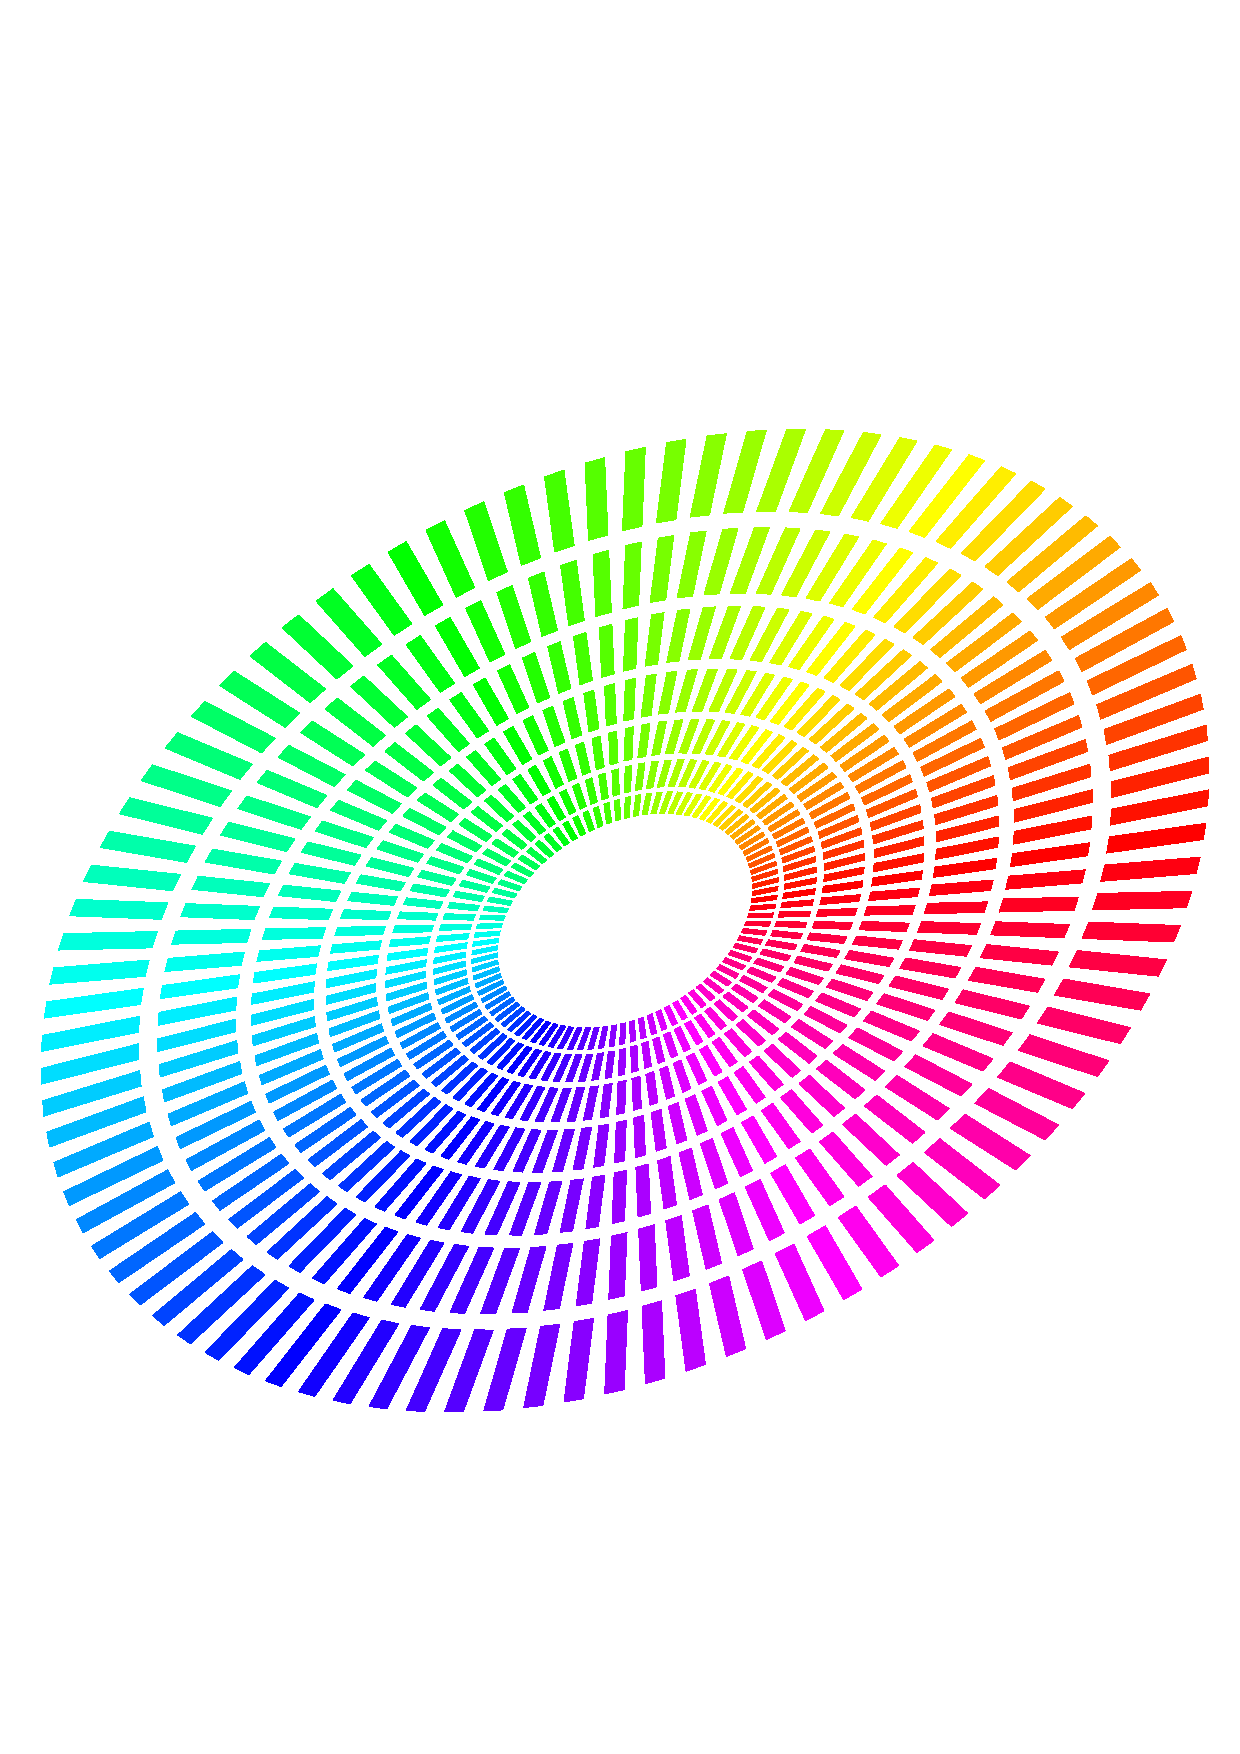
\includegraphics[width=8cm]{figure}
  \caption{A colourful picture.}
  \label{Figure:figex}
\end{figure}

This page shows you a subfigure example in \fref{Figure:figsubex}.
\begin{figure}[!htb]
  \centering
  \subfigure[The left caption]{
    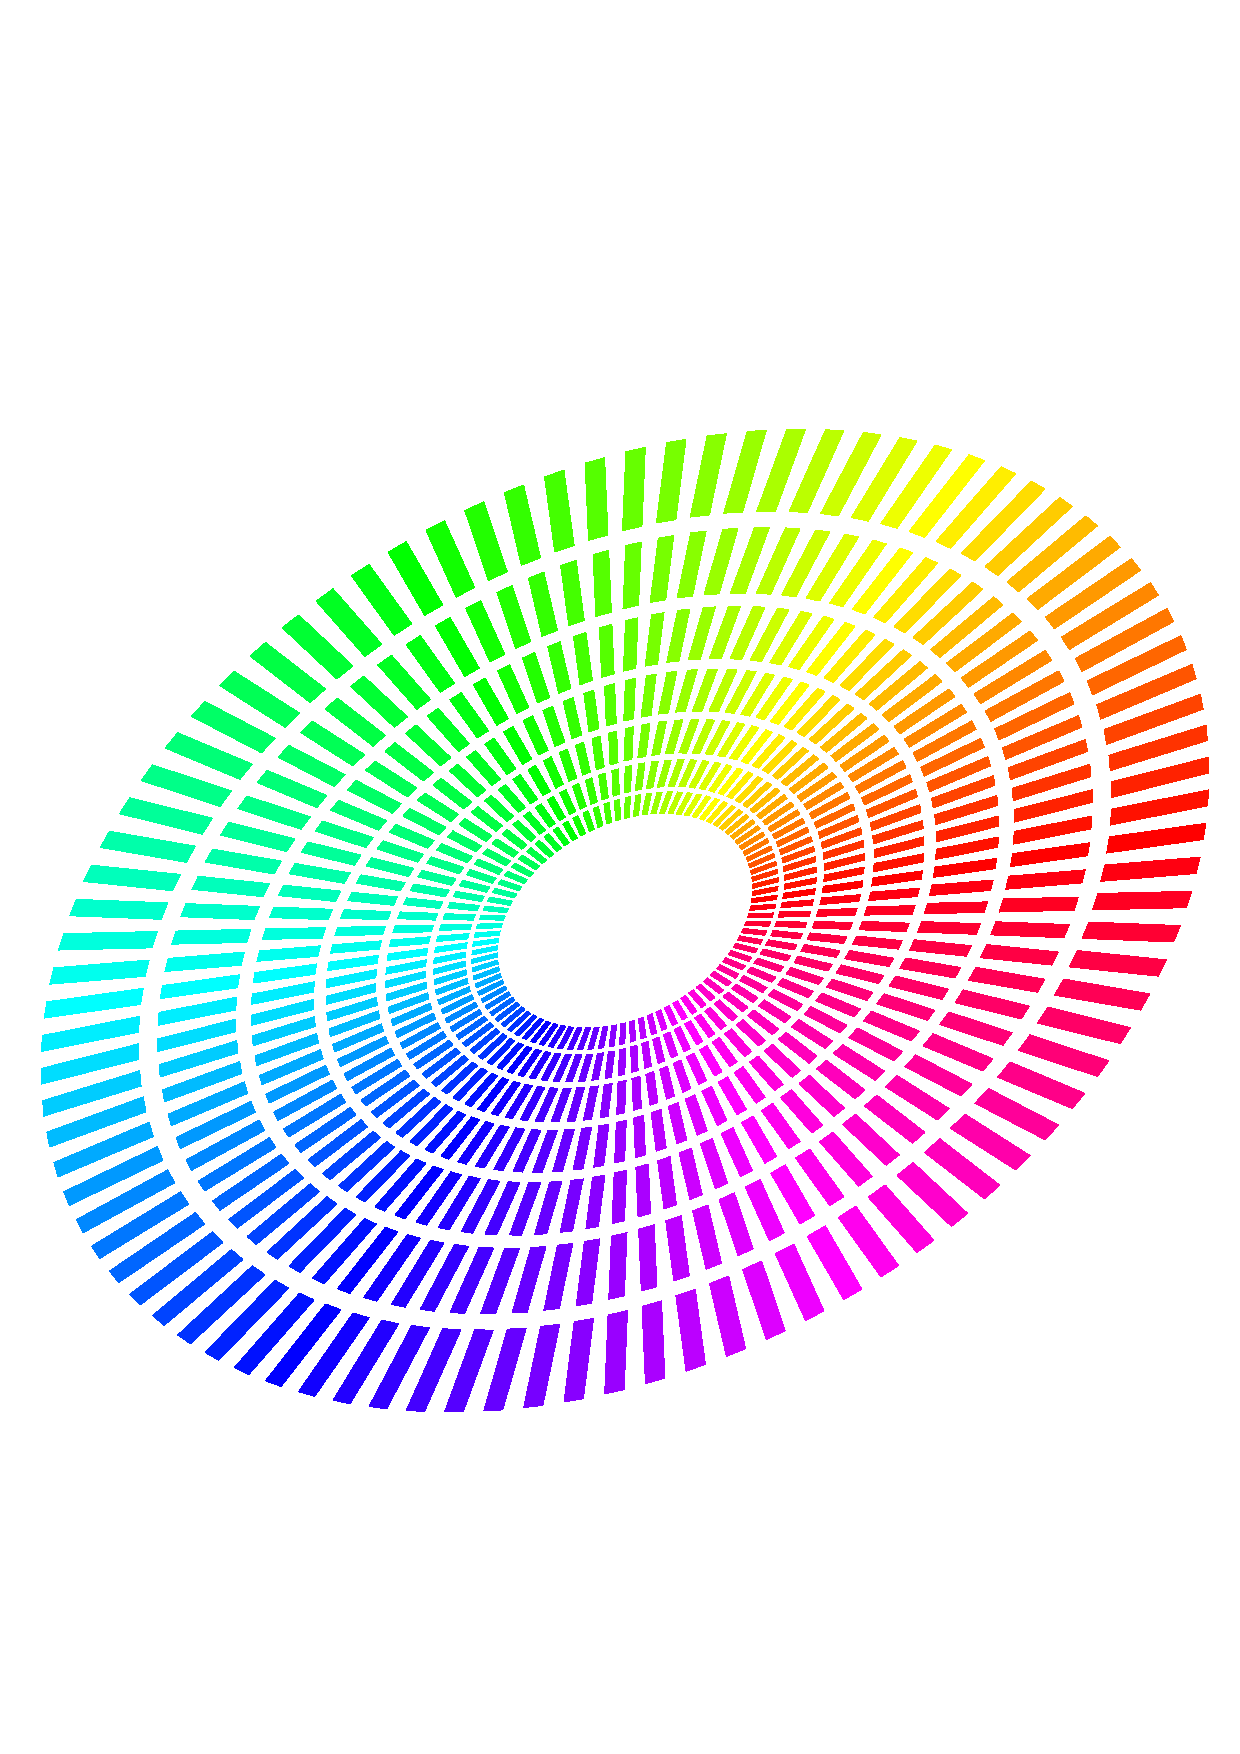
\includegraphics[width=4.2cm]{figure}
    \label{Figure:figsubex:left}
  }
  \subfigure[The right caption]{
    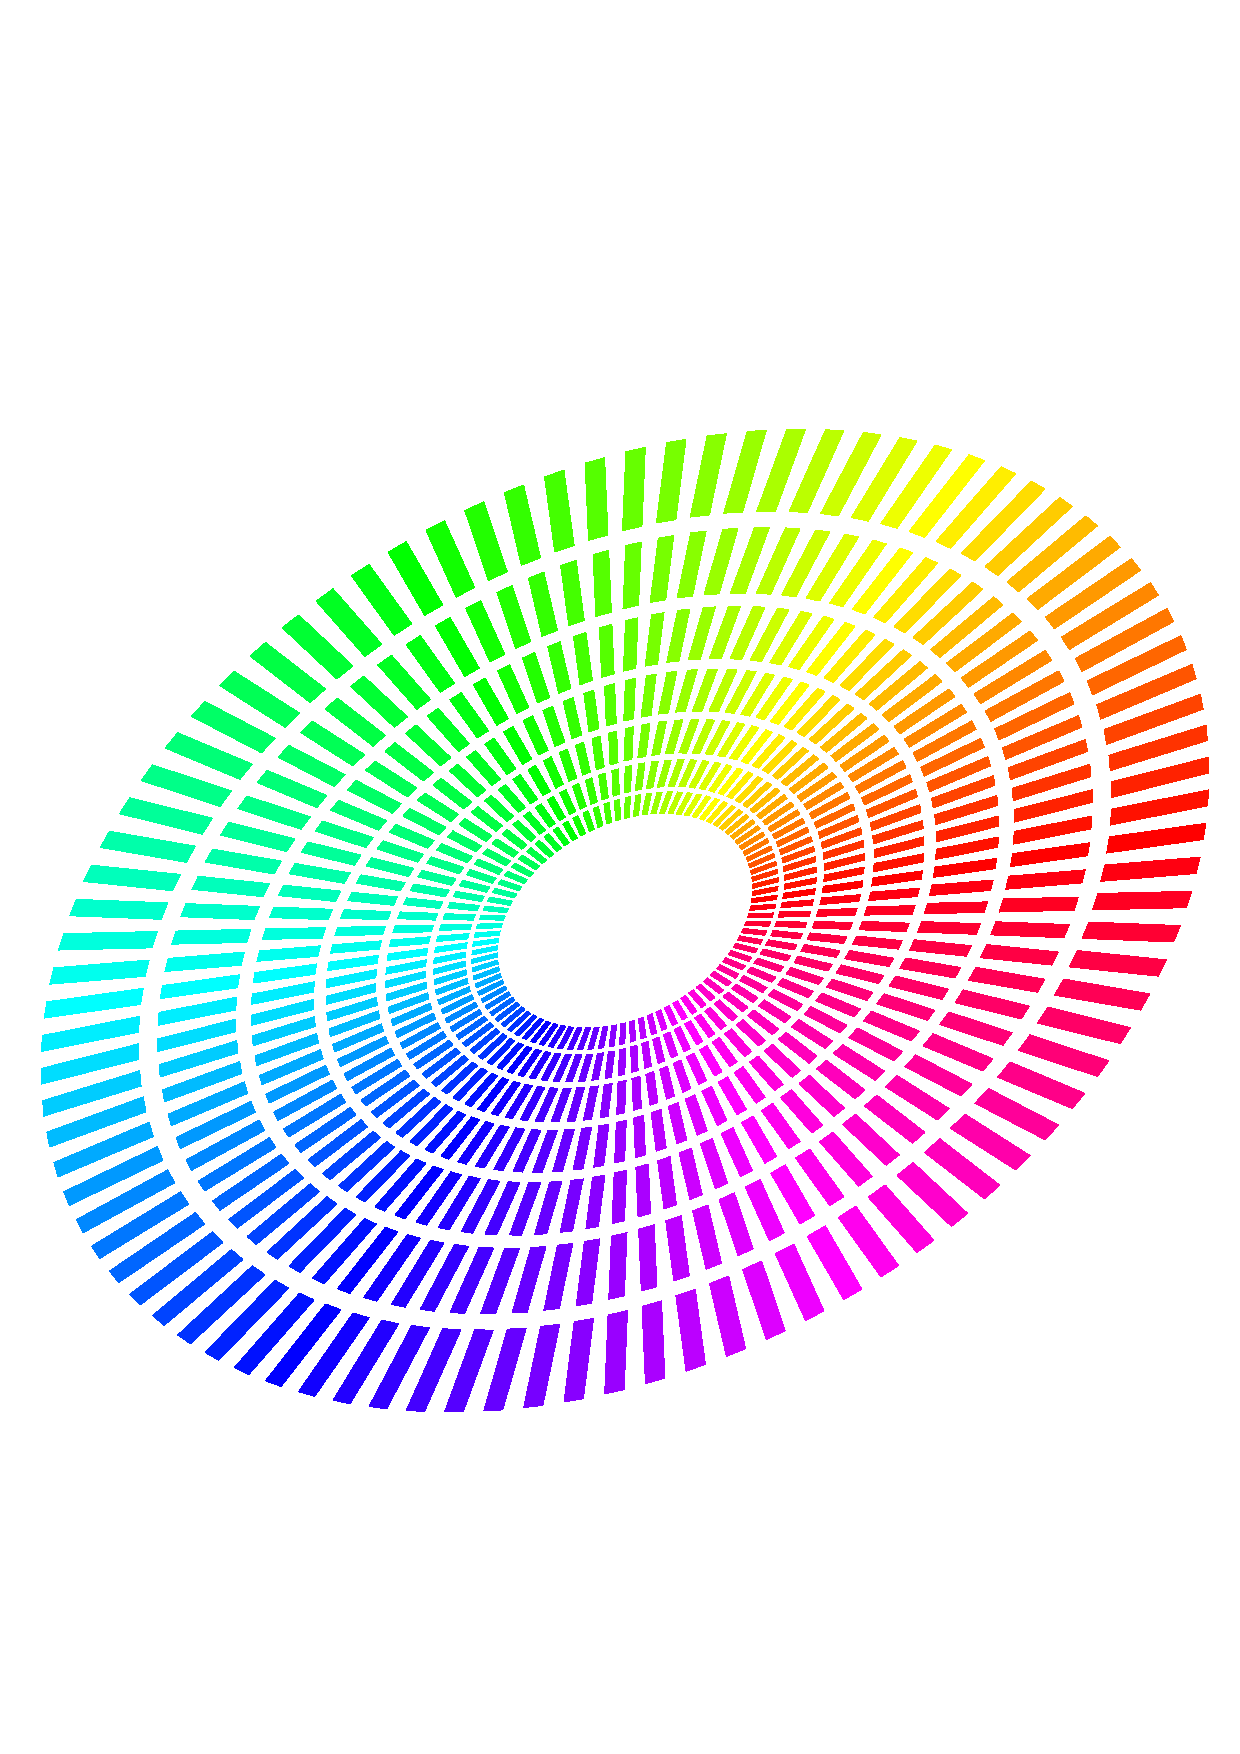
\includegraphics[width=4.2cm]{figure}
    \label{Figure:figsubex:right}
  }
  \caption{A doubly colourful picture.}
  \label{Figure:figsubex}
\end{figure}
\fi